\chapter{\ifenglish Introduction\else บทนำ\fi}

\section{\ifenglish Objectives\else วัตถุประสงค์\fi}
\begin{enumerate}
    \item เพื่อนำความรู้ทั้ง Frontend (การพัฒนาหน้าบ้าน) และ Backend (การพัฒนาหลังบ้าน/ฐานข้อมูล) มาพัฒนาโปรเจกต์หรือระบบจริงขององค์กร
    \item เพื่อฝึกฝนการใช้งานเครื่องมือ (Tools) เฟรมเวิร์ก (Frameworks) และเทคโนโลยีที่ทันสมัยและเป็นที่ยอมรับในภาคอุตสาหกรรม
    \item เพื่อฝึกฝนการทำงานร่วมกับบุคลากรในสายงานที่เกี่ยวข้อง การสื่อสารในสภาพแวดล้อมการทำงานจริง การวางแผนงานและการจัดการความรับผิดชอบภายใต้กรอบเวลาที่กำหนด
    \item เพื่อให้นักศึกษาสามารถวิเคราะห์ วินิจฉัย และหาแนวทางแก้ไขปัญหาทางเทคนิคที่เกิดขึ้นกับระบบจริงได้อย่างเป็นระบบและมีประสิทธิภาพ
\end{enumerate}

\section{\ifenglish Project scope\else ขอบเขตของรายงาน\fi}
รายงานฉบับนี้ครอบคลุมการปฏิบัติงานสหกิจศึกษาในตำแหน่ง Fullstack Developer ณ บริษัท จีเอเบิล จำกัด (G-ABLE Company Limited) โดยเนื้อหาครอบคลุมงานพัฒนาเว็บแอปพลิเคชันทั้งส่วน Frontend และ Backend การออกแบบและพัฒนา API การเชื่อมต่อฐานข้อมูล และการทำงานร่วมกับทีมพัฒนา เพื่อสะท้อนทักษะและประสบการณ์ที่ได้รับจากการฝึกปฏิบัติงานจริง

\section{\ifenglish Expected outcomes\else ประโยชน์ที่ได้รับ\fi}
\begin{enumerate}
    \item ได้พัฒนาความรู้และทักษะด้านการพัฒนาเว็บแอปพลิเคชันทั้งส่วน Frontend และ Backend
    \item ได้เรียนรู้การทำงานจริงในสภาพแวดล้อมขององค์กรด้านเทคโนโลยีสารสนเทศ
    \item ได้เพิ่มพูนประสบการณ์ในการทำงานร่วมกับทีมพัฒนาและการใช้เครื่องมือในการพัฒนาซอฟต์แวร์
    \item ได้เพิ่มพูนประสบการณ์ในการทำงานร่วมกับทีมพัฒนาและการใช้เครื่องมือในการพัฒนาซอฟต์แวร์
    \item ได้นำความรู้ทางวิศวกรรมคอมพิวเตอร์มาประยุกต์ใช้ในการทำงานจริงอย่างมีประสิทธิภาพ
\end{enumerate}

\section{\ifenglish Company History\else ประวัติความเป็นมาของบริษัท\fi}

G-Able \cite{gableWebsite} ก่อตั้งขึ้นในปี 2532 ในชื่อ บริษัท ลอจิก จำกัด โดยเริ่มจากการเป็นตัวแทนจำหน่ายฮาร์ดแวร์และโซลูชันไอที ก่อนจะพัฒนาสู่การเป็นผู้นำด้าน Digital Enabler หรือผู้ให้บริการเทคโนโลยีดิจิทัลแบบครบวงจร. บริษัทได้ขยายธุรกิจไปสู่โซลูชันที่หลากหลาย เช่น Cloud, Cybersecurity, Data Analytics, AI และ Software Development. 

\section{\ifenglish Company Product\else บริการและผลิตภัณฑ์ของบริษัท\fi}
จีเอเบิล เราให้บริการด้านดิจิทัลโซลูชั่นแบบครบวงจร เพื่อช่วยให้องค์กรประสบความสำเร็จในการทำ ดิจิทัล ทรานส์ฟอร์เมชั่น
โซลูชั่นถูกออกแบบและคิดมาให้ใช้งานได้อย่างราบรื่นตั้งแต่การวางแผนเชิงกลยุทธ์ การออกแบบระบบ และการใช้งานระบบ ไปจนถึงโครงสร้างพื้นฐานเครือข่าย การจัดการพื้นที่เก็บข้อมูล ด้วยบริการระดับมืออาชีพ

\section{\ifenglish Organization\else ผู้บริหารของบริษัท\fi}
\begin{table}[ht]
    \centering
    \begin{tabular}{|p{5cm}||p{7cm}|}
        \hline
        \centering \textbf{Name} & \centering \textbf{Position} \tabularnewline
        \hline\hline
        \centering ดร.ชัยยุทธ ชุณหะชา & \centering ประธานเจ้าหน้าที่บริหาร \tabularnewline
        \centering นายอุกฤษฏ์ วงศราวิทย์ & \centering ประธานบริหารสายงานปฏิบัติการ และ ประธานบริหารสายงานโซลูชันและเทคโนโลยี \tabularnewline
        \centering นางนวลนิตย์ หงส์ประภาวงศ์ & \centering ประธานบริหารสายงานขายและพัฒนาธุรกิจ \tabularnewline
        \centering นางสาวรวีรัตน์ สัจจวโรดม & \centering ประธานบริหารสายงานการเงินและกลยุทธ์ \tabularnewline
        \centering นางกิตยานี อัศวาณิชย์ & \centering รองประธานบริหารอาวุโสฝ่ายบัญชีและการเงิน \tabularnewline
        \centering นางฐิติกานต์ กฤษณวิภาคพร & \centering รองประธานบริหารอาวุโสฝ่ายทรัพยากรบุคคล \tabularnewline
        \centering นางกมลทิพย์ สรรพศรี & \centering รองประธานบริหารอาวุโสฝ่ายดิจิทัลและเทคโนโลยีโซลูชัน \tabularnewline
        \centering นางสาววรรณา ศฤงคารบริบูรณ์ & \centering รองประธานบริหารอาวุโสฝ่ายผสมผสานโซลูชั่น \tabularnewline
        \centering นางพิมพ์นารา อธิโชติอนันต์ & \centering รองประธานอาวุโสฝ่ายบัญชี \tabularnewline
        \hline
    \end{tabular}
    \caption{ตารางแสดงตำแหน่งผู้บริหารของบริษัท}
\end{table}
\begin{figure}[ht]
    \begin{center}
        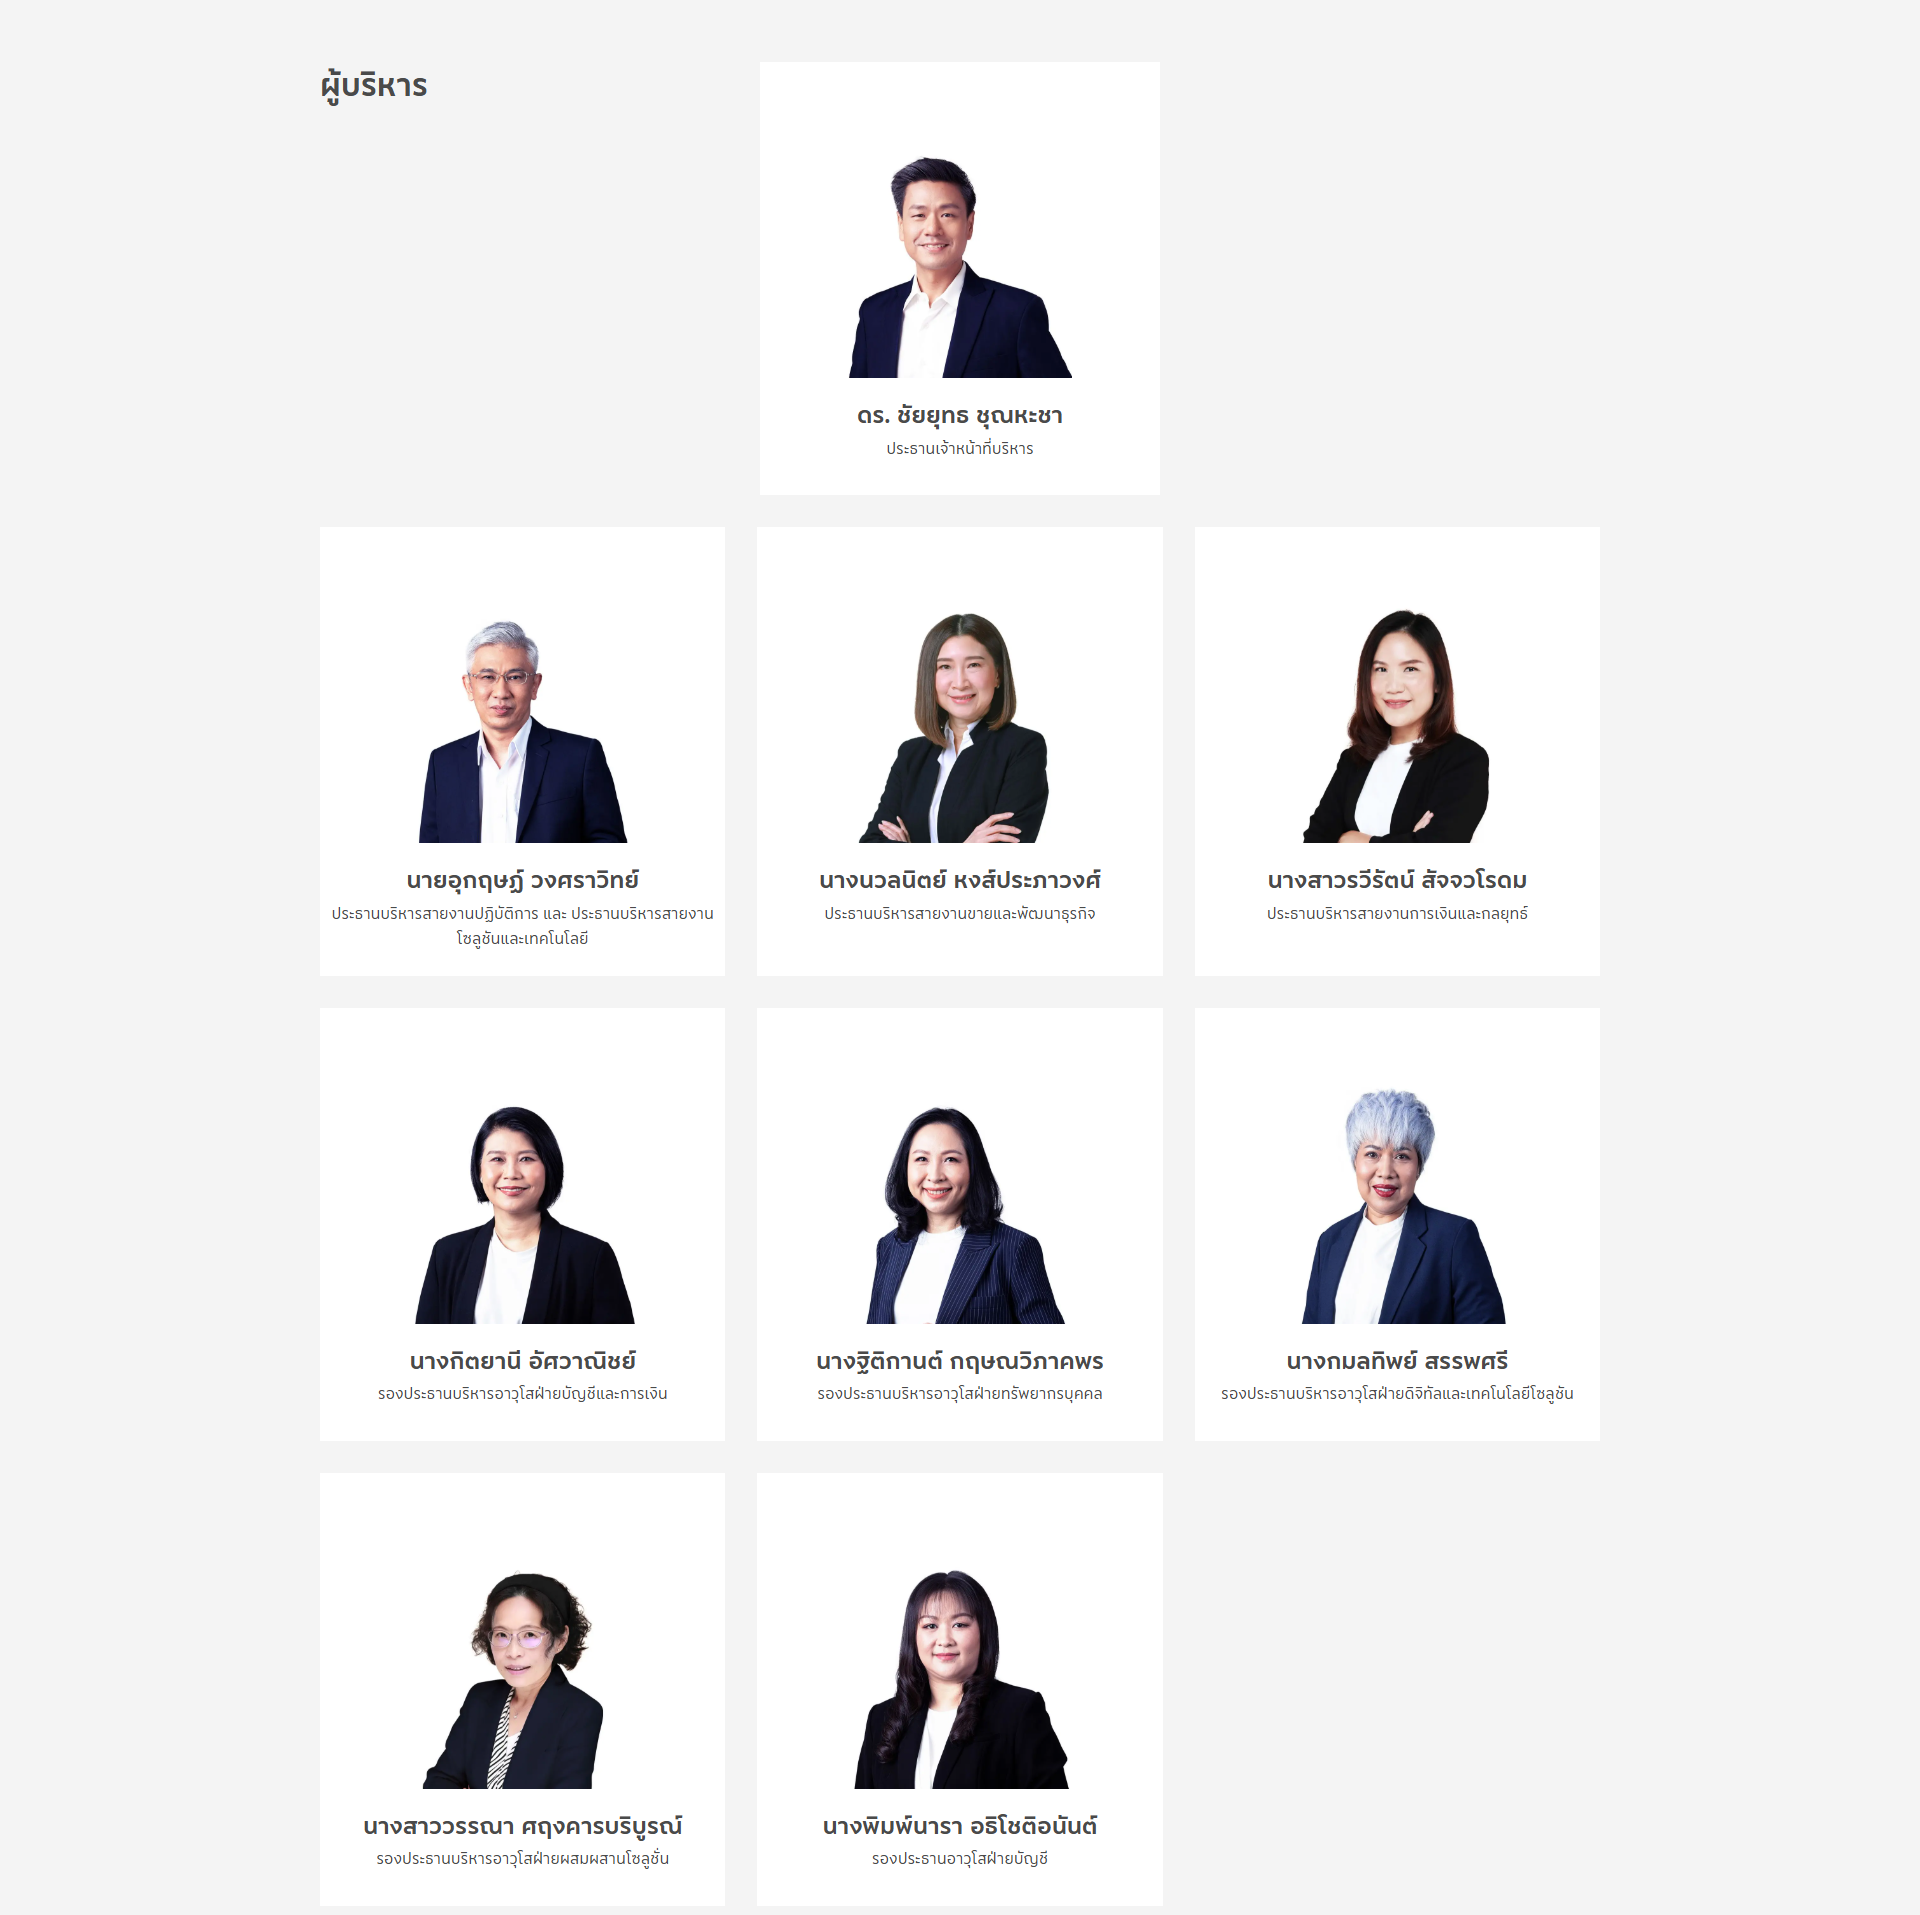
\includegraphics[width=1\linewidth]{./images/g-able-executives.png}
    \end{center}
    \caption[ผู้บริหารและตำแหน่งของบริษัท]{ผู้บริหารและตำแหน่งของบริษัท}
\end{figure}

\clearpage

\section{งบการเงินและงบกำไรขาดทุน}
\subsection{งบการเงิน}
\begin{figure}[ht]
    \begin{center}
        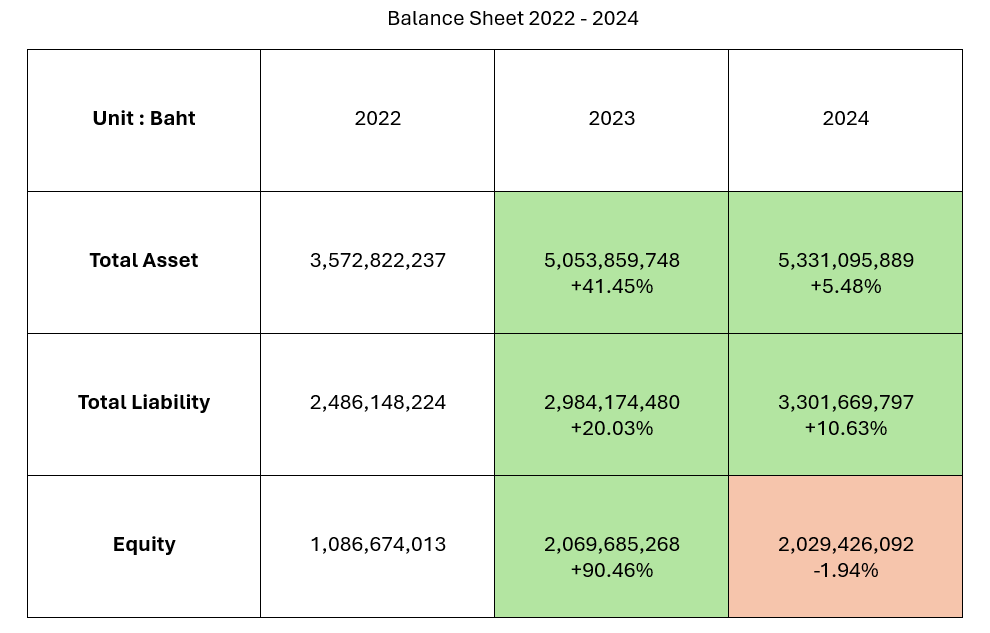
\includegraphics[scale=0.4]{images/balance.png}
    \end{center}
    \caption[งบการเงินย้อนหลังตั้งแต่ก่อตั้งบริษัท]{งบการเงินย้อนหลังตั้งแต่ก่อตั้งบริษัท}
\end{figure}
จากข้อมูลใน \textit{รูปที่ 1.2} จะเห็นได้ว่าบริษัท \textbf{G-Able} มีสินทรัพย์รวมอยู่ที่ 3,573 ล้านบาท ในปี 2022 (ค.ศ. 2022) และเพิ่มขึ้นอย่างรวดเร็วเป็น 5,054 ล้านบาท ในปี 2023 หรือเติบโตประมาณร้อยละ 41.5 ก่อนจะชะลอเป็น 5,331 ล้านบาท ในปี 2024 (+5.5\%) ซึ่งสะท้อนถึงการขยายธุรกิจและการบริหารสินทรัพย์ที่มีประสิทธิภาพ
ในด้านโครงสร้างทุน บริษัทมี \textbf{หนี้สินรวม} เพิ่มจาก 2,486 ล้านบาท เป็น 3,302 ล้านบาท ขณะที่ \textbf{ส่วนผู้ถือหุ้น} เพิ่มจาก 1,087 ล้านบาท เป็น 2,070 ล้านบาท ในปี 2023 ก่อนจะลดเล็กน้อยเหลือ 2,029 ล้านบาท ในปี 2024 แสดงว่าบริษัทสามารถควบคุมหนี้สินได้ดีและยังมีทุนเพียงพอต่อการเติบโต

\textbf{สรุป:} G-Able มีสินทรัพย์สูง โครงสร้างทุนแข็งแรง หนี้สินอยู่ในระดับเหมาะสม และยังคงเติบโตอย่างมั่นคงในระยะยาว

\clearpage


\subsection{งบกำไรขาดทุน}
\begin{figure}[ht]
    \begin{center}
        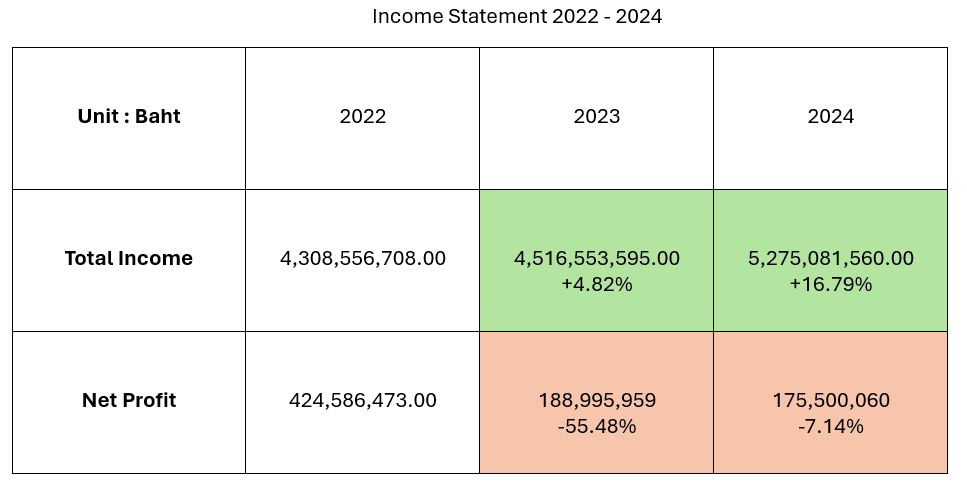
\includegraphics[scale=0.4]{images/income.png}
    \end{center}
    \caption[งบกำไรขาดทุนย้อนหลังตั้งแต่ก่อตั้งบริษัท]{งบกำไรขาดทุนย้อนหลังตั้งแต่ก่อตั้งบริษัท}
\end{figure}

รายได้รวมของบริษัท \textbf{G-Able} ในช่วงปี 2022–2024 เติบโตต่อเนื่องจาก 4,308 ล้านบาท เป็น 5,275 ล้านบาท หรือเฉลี่ยประมาณร้อยละ 10 ต่อปี แสดงถึงการขยายธุรกิจที่แข็งแกร่ง อย่างไรก็ตาม กำไรสุทธิกลับลดลงจาก 425 ล้านบาท ในปี 2022 เหลือ 176 ล้านบาท ในปี 2024 เนื่องจากต้นทุนและค่าใช้จ่ายที่เพิ่มขึ้น

\noindent แนวโน้มในอีก 2–3 ปีข้างหน้า คาดว่ารายได้จะยังเติบโตได้ราวร้อยละ 8–12 ต่อปี โดยอาจแตะระดับ 6,500–7,500 ล้านบาท ขณะที่กำไรสุทธิอาจทรงตัวหรือลดลงเล็กน้อย หากยังไม่สามารถควบคุมต้นทุนได้อย่างมีประสิทธิภาพ ทั้งนี้ การเพิ่มสัดส่วนรายได้จากบริการซอฟต์แวร์และโซลูชันที่มีกำไรสูง จะเป็นกุญแจสำคัญต่อการเติบโตในอนาคต

\clearpage


\section{หน้าที่ของหน่วยงานที่ได้มาสหกิจ}
ในตำแหน่ง Full Stack Developer ที่บริษัท G-ABLE หน้าที่หลักของคือการพัฒนาและปรับปรุงระบบทั้งส่วนหน้า (Front-end) และส่วนหลัง (Back-end) ของเว็บแอปพลิเคชัน โดยมุ่งเน้นให้ระบบทำงานได้อย่างมีประสิทธิภาพและตอบสนองต่อความต้องการของผู้ใช้

นอกจากนี้ ยังได้ทำงานร่วมกับทีม UX/UI เพื่อปรับปรุงประสบการณ์การใช้งานของผู้ใช้ (User Experience) และออกแบบส่วนติดต่อผู้ใช้ (User Interface) ให้ใช้งานได้สะดวกและสวยงาม รวมถึงทำงานร่วมกับทีม QA (Quality Assurance) เพื่อทดสอบ ตรวจสอบ และแก้ไขข้อผิดพลาดของระบบก่อนนำขึ้นใช้งานจริง เพื่อให้มั่นใจว่าระบบมีความถูกต้อง เสถียร และพร้อมใช้งานตามมาตรฐานของบริษัท
